\documentclass{subfile}

\begin{document}
  \section{Simulation Result}
  \subsection{Prediction on Termination on SIS and SIRS Epidemic Simulation Model}
  Since SIS and SIRS epidemic model takes a long time to terminate, and is not able to terminate within 100 iterations, prediction of termination is done using regression. The regression is based on 1 observation.

  \paragraph{Observation 1: }The decrease of peak infected value follows a concave up curve. In infected graphs of SIRS and SIS epidemic models, the peak decreases and when linked up, forms a concave up curve.

  \begin{center}
    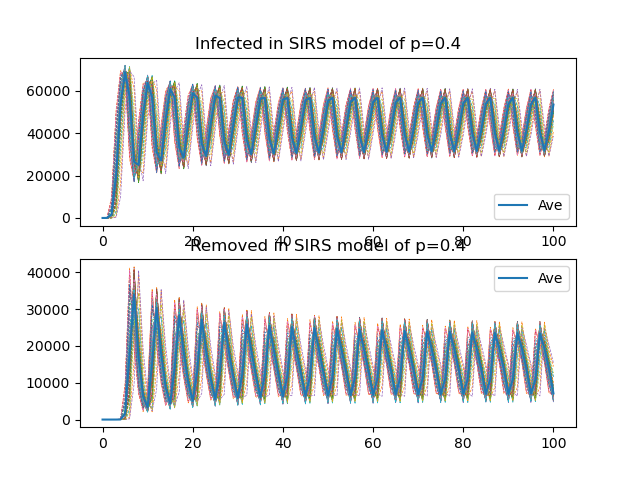
\includegraphics[scale=0.4]{sirsp04r1i3s3}
    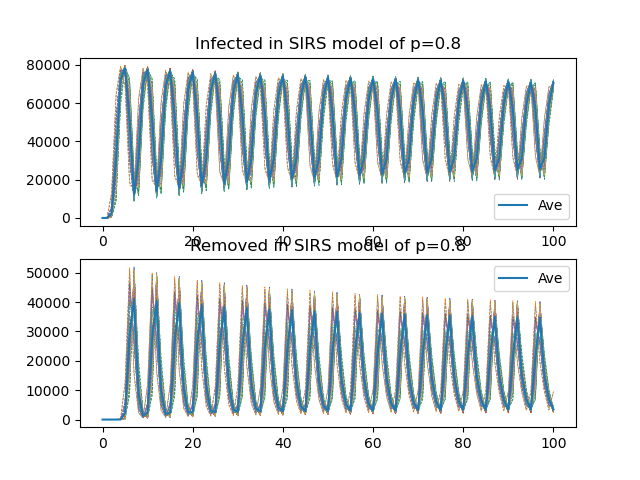
\includegraphics[scale=0.4]{sirsp08r1i3s3}
    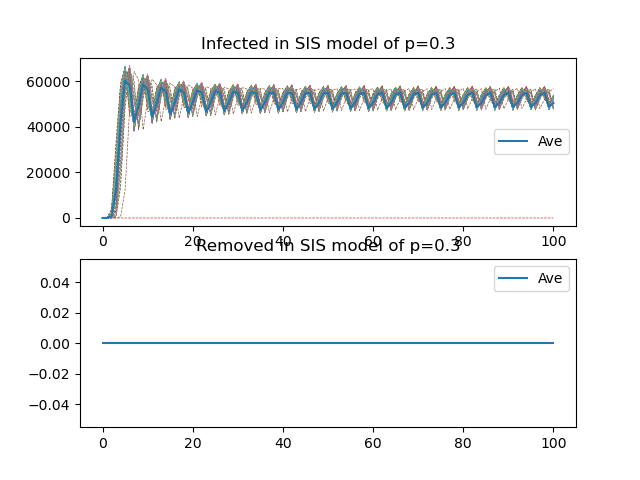
\includegraphics[scale=0.4]{sisp03r1i3s3}
    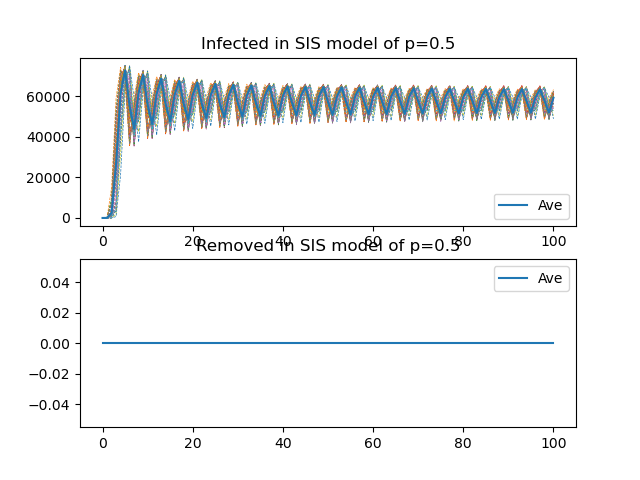
\includegraphics[scale=0.4]{sisp05r1i3s3}
    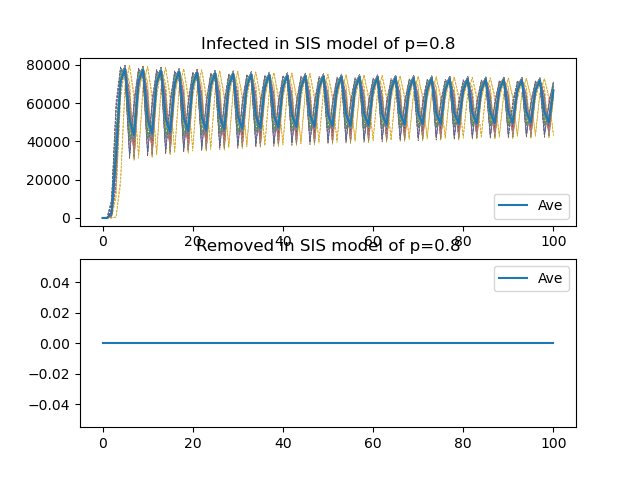
\includegraphics[scale=0.4]{sisp08r1i3s3}\\
  \end{center}
  \begin{figure}[h!]
  \centering
    \caption{Miniature graphs of SIRS and SIS Epidemic Model Simulation Result}
  \end{figure}

  Therefore, an educated geuss that the decay follows the logarithmic model \(y=w_1 log(x) + w_0\) is made. SIS and SIRS data are preprocessed by logarithmic transformation for linear regression for epidemic termination prediction.

  \begin{tabular}{cc}
    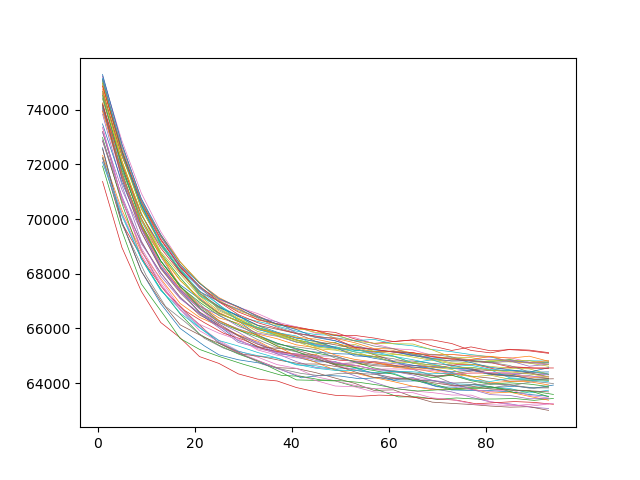
\includegraphics[scale=0.5]{SISp05chaos} & 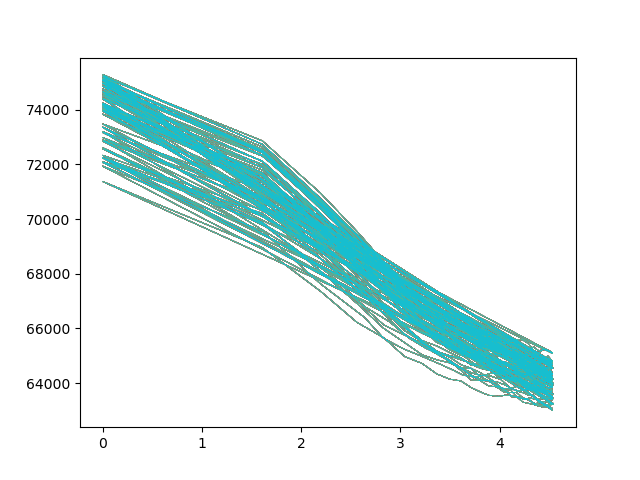
\includegraphics[scale=0.5]{logTrSISp05}\\
    Raw SIS peak value diagram & Log transform processed SIS peak value diagram\\
    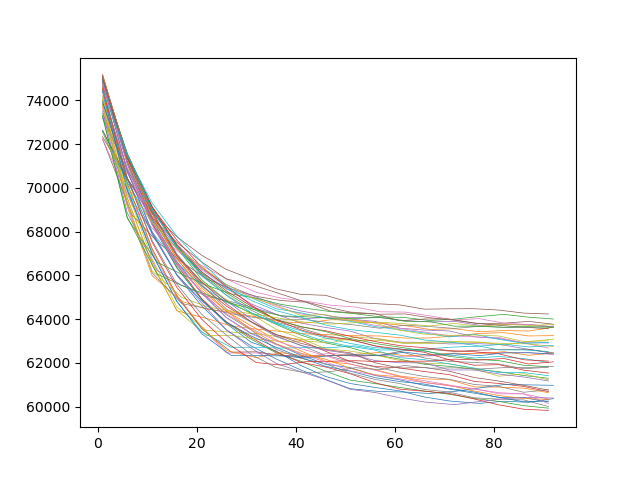
\includegraphics[scale=0.5]{SIRSp05chaos} & 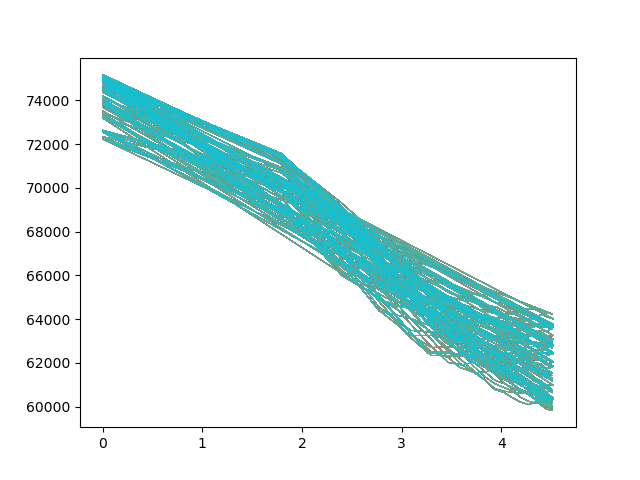
\includegraphics[scale=0.5]{logTrSIRSp05}\\
    Raw SIRS peak value diagram & Log transform processed SIRS peak value diagram\\
  \end{tabular}

  The result shows that the decay of peak values follows logarithmic model. Therefore a probable upper bound of termination of SIRS and SIS epidemic can be made using logarithmic regression.

  \subsection{Observation on Effect of Infection Probability}
  Model Simulation Parameters: \(i=3, r=1, s=3\)

  \subsubsection{SIR Simulation Result}
  \begin{tabular}{|l|l|l|l|l|l|l|l|l|l|l|}
    \hline
    SIR & p=0.1 & p=0.2 & p=0.3 & p=0.4 & p=0.5 & p=0.6 & p=0.7 & p=0.8 & p=0.9 & p=1.0\\
    \hline
    \makecell{Avg.\\Termination\\(\(t\)):} & 19.12 & 17.58 & 16.41 & 15.37 & 14.28 & 13.7 & 13.0 & 12.08 & 11.6 & 11.37\\
    \hline
    \makecell{Avg.\\Fraction of\\ Infected:} & 0.66472 & 0.85094 & 0.92685 & 0.96445 & 0.98348 & 0.99281 & 0.99729 & 0.99925 & 0.99991 & 1.0\\
    \hline
  \end{tabular}

  \subsubsection{SIRS Simulation Result}
  \begin{tabular}{|l|l|l|l|l|l|l|l|l|l|l|}
    \hline
    SIRS & p=0.1 & p=0.2 & p=0.3 & p=0.4 & p=0.5 & p=0.6 & p=0.7 & p=0.8 & p=0.9 & p=1.0\\
    \hline
    \makecell{Predicted Avg.\\ Termination(\(t\))}: & \(e^{12.378}\) & \(e^{16.010}\) & \(e^{23.423}\) & \(e^{23.639}\) & \(e^{23.153}\) & \(e^{23.494}\) & \(e^{26.516}\) & \(e^{31.904}\) & \(e^{40.203}\) & 12.0\footnote{actual average termination is taken as when p=1.0, the SIRS model simulations succeeded in terminating}\\
    \hline
  \end{tabular}
\end{document}
